\begin{center}
	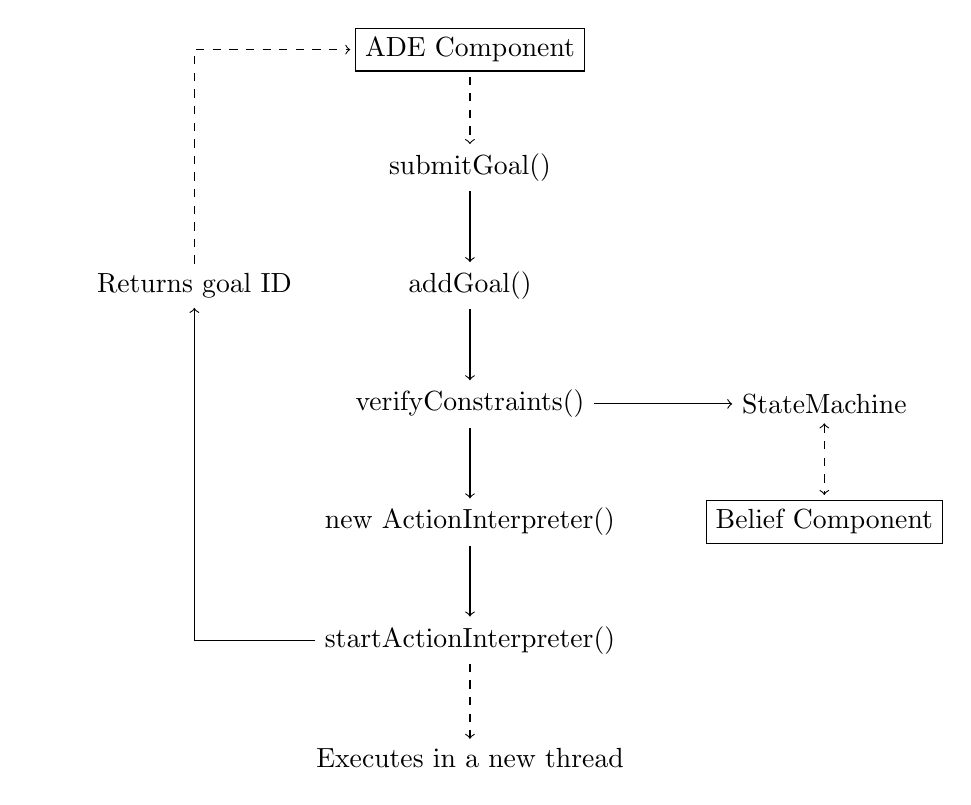
\begin{tikzpicture}[node distance=1.5cm,every node/.style={fill=white},align=center]
	% Specification of nodes (position, etc.)
	\node (start)				[draw, outer sep=2pt]	{ADE Component};
	\node (submitGoal)	[below of=start]						{submitGoal()};
	\node (addGoal)			[below of=submitGoal]				{addGoal()};
	\node (verifyCstr)	[below of=addGoal]   				{verifyConstraints()};
	\node (stateMachine)[right of=verifyCstr, xshift=3cm]
																									{StateMachine};
	\node (belief)			[below of=stateMachine, draw, outer sep=2pt]
																									{Belief Component};
	\node (newAI)				[below of=verifyCstr]  			{new ActionInterpreter()};
	\node (startAI)			[below of=newAI]						{startActionInterpreter()};
	\node (runAI)				[below of=startAI]					{Executes in a new thread};
	\node (return)			[left of=addGoal, xshift=-2cm, text width=4cm]	
																									{Returns goal ID};

	% Specification of lines between nodes specified above
	% with aditional nodes for description 
	\draw[dashed, ->]		(start) -- (submitGoal);
	\draw[->]						(submitGoal) -- (addGoal);
	\draw[->]						(addGoal) -- (verifyCstr);
	\draw[->]						(verifyCstr) -- (stateMachine);
	\draw[dashed, <->]	(stateMachine) -- (belief);
	\draw[->]						(verifyCstr) -- (newAI);
	\draw[->]						(newAI) -- (startAI);
	\draw[->]						(startAI) -| (return);
	\draw[dashed, ->]		(return) |- (start);
	\draw[dashed, ->]		(startAI) -- (runAI);
	\end{tikzpicture}
\end{center}